\documentclass[onecolumn, aps, nofootinbib, prd, preprint, floats, floatfix, amsmath, amssymb, superscriptaddress, preprintnumbers]{revtex4-2}
\PassOptionsToPackage{dvipsnames}{xcolor}
\usepackage{slashed}
\usepackage{graphicx}
\usepackage{subcaption}
\usepackage{dcolumn}
\usepackage{bm}
\usepackage{amssymb}
\usepackage{tikz}
\usepackage{tikz-feynman}
%\usepackage{xcolor}
\usepackage[utf8]{inputenc}
% \usepackage[OT1]{fontenc}
\usepackage{yfonts,amsmath,amsthm,amsfonts,amssymb,amscd, ulem}
\usepackage{enumerate}
\usepackage{fancyhdr}
\usepackage{mathtools}
\usepackage{amsmath}
\usepackage{autobreak}
\usepackage{mathrsfs}
\usepackage{cancel}
\usepackage{slashed}
\usepackage{bigints}
\usepackage[flushleft]{threeparttable}
\usepackage[colorlinks=true, citecolor=purple, linkcolor=blue]{hyperref}
\usepackage{url}
\usepackage{makecell,booktabs}
\usepackage{braket}
\usepackage{relsize}
\usepackage{multirow}
\usepackage{verbatim}
\usepackage{txfonts}
\usepackage{slashed}
\usepackage{upgreek}
\usepackage{extarrows}
\usepackage{array}
\usepackage{appendix}
\usepackage[T1]{fontenc}
\usepackage{setspace}
\usepackage{subcaption}
\newcommand{\GJH}[1]{\textcolor{blue} {GJH: #1}}
\newcommand{\jl}[1]{\textcolor{orange} {jl: #1}}
\newcommand{\WXP}[1]{\textcolor{purple} {WXP: #1}}
\newcommand{\zb}[1]{{\color{blue} {#1}}}
\usepackage{xcolor}
\definecolor{c1}{HTML}{1bd1a5}
\usepackage{graphicx}   % 引入图片
\usepackage{caption}    % 总 caption 支持
\usepackage{subcaption} % 子图支持
\usepackage{subcaption}
\usepackage{cleveref}
\usepackage{orcidlink}
\captionsetup{justification=raggedright, singlelinecheck=false}


\begin{document}

\title{An Axial $U_A(1)_{L_\mu-L_\tau}$ Gauge Boson: UV Completion and Experimental Searches}

\author{Rundong Fang}
\email{xxxxx}
\affiliation{School of Physics and State Key Laboratory of Nuclear Physics and Technology, Peking University, Beijing 100871, China}

\author{Jinhui Guo}
\email{guojh23@buaa.edu.cn}
\affiliation{School of Physics, Beihang University, Beijing 100191, China}

\author{Ming Li \orcidlink{0009-0007-7322-010X}}
\email{by2419116@buaa.edu.cn}
\affiliation{School of Physics, Beihang University, Beijing 100191, China}

\author{Jia Liu \orcidlink{0000-0001-7386-0253}}
\email{jialiu@pku.edu.cn}
\affiliation{School of Physics and State Key Laboratory of Nuclear Physics and Technology, Peking University, Beijing 100871, China}
\affiliation{Center for High Energy Physics, Peking University, Beijing 100871, China}

\author{Xiao-Ping Wang \orcidlink{0000-0002-2258-7741} }
\email{hcwangxiaoping@buaa.edu.cn}
\affiliation{School of Physics, Beihang University, Beijing 100191, China}

\author{Yiheng Xiong \orcidlink{0009-0006-1377-1228} }
\email{yihenghht@buaa.edu.cn}
\affiliation{School of Physics, Beihang University, Beijing 100191, China}

\maketitle
\tableofcontents

\section{Introduction}
\label{sec:introduction}

Light neutral spin-one bosons provide a minimal and experimentally accessible extension of the Standard Model (SM). Besides the kinetically mixed dark photon~\cite{Holdom:1985ag}, anomaly-free differences of lepton-flavor numbers single out predictive leptophilic gauge symmetries, of which $U(1)_{L_\mu-L_\tau}$ is the best studied~\cite{Foot:1990mn,He:1990pn,He:1991qd}. In its conventional realization, the new boson couples vectorially to charged muons and taus and left-handedly to their neutrinos. This economical structure has been connected to neutrino masses and mixing, a positive contribution to the muon anomalous magnetic moment, dark-sector interactions, and multi-lepton collider signatures~\cite{Baek:2001kca,Ma:2001md,Heeck:2011wj,Harigaya:2013twa,Altmannshofer:2014cfa,Crivellin:2015mga,Altmannshofer:2016brv}. It also defines the standard two-parameter $(m_{Z'},g')$ benchmark against which most searches are reported.

The corresponding experimental program now spans several complementary observables. Neutrino trident production provides a particularly robust low-mass constraint~\cite{Altmannshofer:2014pba}, while general collider studies identified multi-lepton final states as the natural probes of leptophilic vectors~\cite{delAguila:2014soa}. At electron colliders, final-state radiation from a muon gives either a visible four-muon resonance or an invisible recoil-mass signal; these channels were developed in phenomenological studies~\cite{Araki:2017wyg,Brown:2024jah} and pursued by BaBar and Belle II~\cite{BaBar:2016sci,Belle-II:2019qfb,Belle-II:2022yaw,Belle-II:2024wtd}. At the LHC, CMS searched for $Z\to\mu^+\mu^-Z'$ with $Z'\to\mu^+\mu^-$~\cite{CMS:2018yxg}, whereas the NA64 muon program probes invisibly decaying mediators through missing energy and momentum~\cite{NA64:2024klw}; proposed muon missing-momentum experiments extend the same strategy~\cite{Kahn:2018cqs}. These results constitute essential experimental anchors, but their published coupling contours assume the conventional vector current, together with benchmark-dependent widths and branching fractions. They therefore cannot in general be read as model-independent limits on an axial mediator.

The distinction is physical rather than semantic. Replacing the charged-lepton vector current by an axial current changes which SM four-fermion coefficient is shifted in neutrino trident production, reverses the role of $(g-2)_\mu$ by producing a negative and longitudinally enhanced contribution, and can alter production kernels, decay widths, and angular acceptance in visible or missing-energy searches. It also removes some familiar vector-model intuition: in the absence of an additional ultraviolet source, a purely axial charged-lepton current does not generate the ordinary parity-even photon--$A'$ kinetic mixing at one loop. Existing studies of light axial forces, anomaly-free axial $Z'$ theories, nuclear-transition anomalies, and axial muon-force searches have exposed parts of this phenomenology and its consistency conditions~\cite{Kahn:2016vjr,Ismail:2016tod,Kozaczuk:2016nma,Hicyilmaz:2022owb,Batell:2011qq,Davoudiasl:2012ag,Fayet:2020bmb,Baruch:2022esd,Fayet:2024ddk}. Recent flavor-specific chiral and universal-seesaw constructions further emphasize that a genuine axial gauge interaction is inseparable from its symmetry-breaking scalars and heavy-fermion sector~\cite{Prajapati:2026tfv,Dutta:2026dnf}. What remains missing is a unified axial $L_\mu-L_\tau$ treatment in which this UV structure and the experimental reinterpretation are developed together.

We address this gap with an anomaly-free, leptophilic $U_A(1)_{L_\mu-L_\tau}$ construction in which opposite left- and right-handed charged-lepton charges produce an axial current, while the neutrino current remains left-handed. Because the symmetry forbids the diagonal SM Yukawa operators, a singlet scalar and heavy vector-like leptons generate the charged-lepton masses and correlate the low-energy theory with the symmetry-breaking sector. On this UV-consistent footing, we derive the mass-basis gauge and scalar interactions, calculate neutrino trident production with finite $m_\mu$, reinterpret invisible pion-decay and muon-beam missing-energy searches, and clarify the axial $(g-2)_\mu$ bound and its relation to the UV parameter space. We also compare axial and vector signals at a muon collider, distinguishing approximately rescalable rate observables from angular distributions that retain direct sensitivity to chirality.

This paper is organized as follows. In Sec.~\ref{sec:model-setup} we present the UV model and its mass-basis interactions. In Sec.~\ref{sec:phenomenology} we derive and reinterpret the relevant low-energy and intensity-frontier constraints. In Sec.~\ref{sec:muon-collider} we study future muon-collider probes and axial--vector discrimination. We summarize our results in Sec.~\ref{sec:conclusion}.


\section{Model Setup}
\label{sec:model-setup}

\subsection{An anomaly-free axial $U(1)_{L_\mu-L_\tau}$ completion}

The conventional $U(1)_{L_\mu-L_\tau}$ extension is anomaly free with the
Standard Model (SM) fermion content and gives vector couplings to charged
leptons.  An axial interaction instead requires opposite charges for the
left- and right-handed charged leptons.  This assignment forbids the SM
Yukawa operators $\bar L_\mu H\mu_R$ and $\bar L_\tau H\tau_R$; hence a
consistent axial model must explain charged-lepton mass generation as well as
gauge-anomaly cancellation.

We extend the SM gauge group by $U(1)_A\equiv
U(1)_{L_\mu-L_\tau}$ and introduce two vector-like charged leptons,
$E_\mu$ and $E_\tau$, and a complex SM-singlet scalar $S$.  The scalar vacuum
expectation value (VEV) breaks $U(1)_A$, while the heavy leptons generate the
muon and tau masses through a universal-seesaw mechanism.  Our charge
convention is given in Table~\ref{tab:charge-assignment}.  Only the product of
the gauge coupling and the charge normalization is physical; we define
$g_X\equiv g_{A'}Q_\ell$ and later set $Q_\ell=1$.

\begin{table}[htbp]
    \centering
    \begin{tabular}{cccc}
    \hline
    Field & $SU(2)_L$ & $U(1)_Y$ & $U_A(1)'_{L_\mu-L_\tau}$ \\
    \hline
    $L_{\mu}=\left(\nu_{\mu}, \mu_L\right)^T$ & $\mathbf{2}$ & $-1 / 2$ & $Q_{\ell}$ \\
    \hline
    $\mu_R$ & $\mathbf{1}$ & -1 & $-Q_\ell$ \\
    \hline
    $E_\mu\left(E_{\mu L}, E_{\mu R}\right)$ & $\mathbf{1}$ & -1 & $Q_\ell$\\
    \hline
    $L_{\tau}=\left(\nu_{\tau}, \tau_L\right)^T$ & $\mathbf{2}$ & $-1 / 2$ & $-Q_\ell$ \\
    \hline
    $\tau_R$ & $\mathbf{1}$ & -1 & $Q_\ell$ \\
    \hline
    $E_\tau\left(E_{\tau L}, E_{\tau R}\right)$ & $\mathbf{1}$ & -1 & -$Q_\ell$\\
    \hline
    $H$ & $\mathbf{2}$ & $1 / 2$ & 0 \\
    $S$ & $\mathbf{1}$ & 0 & $Q_S=2Q_\ell$\\
    \hline
    \end{tabular}
    \caption{Field content and $U_A(1)'_{L_\mu-L_\tau}$ charge assignment for the axial $L_\mu-L_\tau$ construction. The electron sector is neutral under $U_A(1)'_{L_\mu-L_\tau}$.}
    \label{tab:charge-assignment}
\end{table}

An important feature of this construction is that all gauge and mixed gravitational anomalies cancel exactly, even though each lepton generation is individually chiral under the new gauge symmetry. As an illustration, the cubic anomaly satisfies \cite{Ismail:2016tod}
\begin{equation}
\mathcal{A}_{[U_A(1)'_{L_\mu-L_\tau}]^3}
\propto
2(+1)^3
-(-1)^3
+2(-1)^3
-(+1)^3
=0,
\end{equation}
where the factor of two originates from the $SU(2)_L$ doublets and the right-handed fermions contribute with the opposite sign. The mixed gravitational anomaly cancels in the same manner. Consequently, the model provides a renormalizable and anomaly-free realization of an axial $U(1)_{L_\mu-L_\tau}$ gauge symmetry.



With the field content fixed by Table~\ref{tab:charge-assignment}, the renormalizable Lagrangian of the UV-complete theory is given by
\begin{equation}\label{eq:Lagrangian}
\begin{aligned}
\mathcal{L}_{UV}\supset& -\frac{1}{4}A'_{\alpha\beta}A'^{\alpha\beta}+\sum_{\alpha=\mu,\tau}\left(i\bar{L}_\alpha \gamma^\nu D_{\nu} L_\alpha + i\bar{\ell}_{\alpha R} \gamma^\nu D_{\nu}\ell_{\alpha R} + i\bar{E}_{\alpha}\gamma^\nu D_{\nu} E_{\alpha}\right)  \\
& -y_\mu \bar L_\mu H E_{\mu R} -\lambda_\mu S \bar E_{\mu L}\ell_{\mu R} -M_{E\mu}\bar E_{\mu L}E_{\mu R} + h.c.\\
&-y_\tau \bar L_\tau H E_{\tau R} -\lambda_\tau S^{*}\bar E_{\tau L}\ell_{\tau R} -M_{E\tau}\bar E_{\tau L}E_{\tau R} + h.c.\\
&+ (D_{\nu}S)^\dagger (D^{\nu}S) - V(S),
\end{aligned}
\end{equation}
where $A'_{\alpha\beta}=\partial_\alpha A'_\beta - \partial_\beta A'_\alpha$ is the field-strength tensor, the covariant derivative is given by $D_\nu = \partial_\nu -ig_Y \frac{Y}{2}B_\nu  -ig_W T^iW_\nu^i - ig_{A'} Q_{A'} A'_\nu$, where $B_\nu$, $W_\nu^i$ and $A'_\nu$ represent the gauge fields for the ${U(1)}_Y$, ${SU(2)}_L$ and ${U_A(1)}_{L_\mu-L_\tau}$ groups, respectively. The constants $g_Y$, $g_W$ and $g_{A'}$ are their associated coupling constants. And, $V(S)$ is the self-interacting potential of $S$. Furthermore, the ordinary diagonal SM Yukawa operator $\bar L_\ell H\ell_R$ is forbidden due to the charge assignment. Consequently, the interactions between charged leptons and Higgs in this model necessarily arise via the new fields, $E$ and $S$. Integrating out the heavy field $E$ at the matching scale $\lambda=M_E$ generates the following dimension-5 effective operators:
\begin{equation}\label{eq:5-d}
    \mathcal{L}_{\text{5-d}} =
    -\frac{c_\mu}{\Lambda} S \bar{L}_\mu H\mu_R
    -\frac{c_\tau}{\Lambda} S^* \bar{L}_\tau H\tau_R
    +h.c.,
\end{equation}
where, in the tree level, $\frac{c_\alpha}{\Lambda}\simeq \frac{y_\alpha \lambda_\alpha}{M_{E\alpha }}$ for $\alpha=\mu,\tau$.

After the electroweak and $U_A(1)_{L_\mu-L_\tau}$ spontaneous symmetry breaking, the scalar fields are given by $H=\frac{1}{\sqrt{2}}\left (\begin{array}{c} 0 \\ v_h+h \end{array}\right)$ and $S=\frac{1}{\sqrt{2}} (v_s + s)$, where $v_{h/s}$ denotes the VEVs of the Higgs and scalar $S$, respectively. The kinetic term
$(D_\nu S)^\dagger(D^\nu S)$ gives the new gauge-boson mass as following
\begin{align}
m_{A'}=|Q_S|g_{A'}v_s=2|Q_\ell|g_{A'}v_s\equiv2|g_X|v_s,
\end{align} 
with $g_X\equiv g_{A'}Q_\ell$. And the mass terms for leptons can be derived as
\begin{equation}
\mathcal{L}_{\mathcal M}=-
\begin{pmatrix}
	\overline{\ell^{\mu}_L},  &
	\overline{E^\mu_L}, &
	\overline{\ell^\tau_L}, &
	\overline{E^\tau_L}
\end{pmatrix}
\begin{pmatrix}
	0 & y_{\mu}v_h/\sqrt2  & 0 & 0 \\
	\lambda_\mu v_s/\sqrt2 & M_{E\mu} & 0 & 0\\
	0 & 0 & 0 & y_{\tau}v_h/\sqrt2\\
    0 & 0 &  \lambda_\tau v_s/\sqrt2 & M_{E\tau}
\end{pmatrix}
\begin{pmatrix}
	\ell^{\mu}_R \\
	E^\mu_R \\
	  \ell^\tau_R \\
	  E^\tau_R \\
\end{pmatrix}
+h.c. = -\bar{\chi}_L \mathcal{M} \chi_R + h.c.
\label{eq:4by4-mass-no-mutau}
\end{equation}
Here, $\chi_L=(\ell^{\mu}_L,E^\mu_L,\ell^\tau_L, E^\tau_L)^T$, $\chi_R=(\ell^{\mu}_R,E^\mu_R,\ell^\tau_R, E^\tau_R)^T$. Because the
$4\times4$ matrix $\mathcal M$ contains independent muon and tau blocks, each
flavor can be diagonalized separately.  It is sufficient to display the muon
block explicitly; the tau block follows by the corresponding change of flavor
labels.  The muon mass term is
\begin{equation}
\mathcal{L}_{\mathcal{M},\mu}
=-\overline{\chi^\mu_L}\,\mathcal{M}_\mu\,\chi^\mu_R+h.c.,
=-\overline{\chi^\mu_L}
\begin{pmatrix}
0 & m_L\\
m_R & M_{E\mu}
\end{pmatrix} \chi^\mu_R+h.c.,
\label{eq:mu-2by2-mass}
\end{equation}
with $\chi^\mu_L=(\ell^\mu_L, E^\mu_L)^T$, $\chi^\mu_R =
(\ell^\mu_R,E^\mu_R)^T$, and $m_L=\frac{y_\mu v}{\sqrt2},
m_R=\frac{\lambda_\mu v_s}{\sqrt2}$. Assuming these mass entries are real, the mass matrix can be bi-orthogonally diagonalized as
\begin{equation}
U_{\mu L}^T\mathcal{M}_\mu U_{\mu R} =
\begin{pmatrix}
m_\mu &0\\
0&m_{E\mu}
\end{pmatrix},~ {\rm with}~
\chi^\mu_L=U_{\mu L} \chi^{\mu \prime}_L~{\rm and}~
\chi^\mu_R=U_{\mu R} \chi^{\mu \prime}_R,
\end{equation}
with $U_{\mu L/\mu R}=\begin{pmatrix}\cos\theta_{\mu L/\mu R} &\sin\theta_{\mu L/\mu R}\\-\sin\theta_{\mu L/\mu R} & \cos\theta_{\mu L/\mu R} \end{pmatrix}$. And the mass eigenvalues are
\begin{equation}
m_{\mu/E\mu}^2=
\frac{1}{2}
\left[
m_L^2+m_R^2+M_{E\mu}^2 \mp
\sqrt{(m_L^2+m_R^2+M_{E\mu}^2)^2-4m_L^2m_R^2}
\right].
\label{eq:exact-masses-2by2}
\end{equation}
The mixing angles can be written as
\begin{equation}
\tan2\theta_{\mu L}= \frac{2m_L M_{E\mu}}{M_{E\mu}^2+m_R^2-m_L^2},
\qquad
\tan2\theta_{\mu R}=\frac{2m_R M_{E\mu}}{m_L^2+M_{E\mu}^2-m_R^2}.
\label{eq:mixing-angles-2by2}
\end{equation}
In the limit $M_{E\mu}\gg m_L, m_R$, to the leading order, the muon block masses and mixing angles can be simplified to
\begin{equation}
\begin{aligned}
    &m_\mu^2\simeq\frac{m_L^2 m_R^2}{M_{E\mu}^2},~ m_{E\mu}^2\simeq M_{E\mu}^2+(m_L^2 + m_R^2)\\
    &\theta_{\mu L}\simeq \frac{m_L}{M_{E\mu}},~ \theta_{\mu R}\simeq \frac{m_R}{M_{E\mu}},
\end{aligned}
\end{equation}
The first relation shows explicitly how the light muon mass is suppressed by
the heavy vector-like mass.  It also agrees with the mass obtained from the
dimension-5 operator in Eq.~\eqref{eq:5-d} after symmetry breaking.  The last
two relations show that the same hierarchy suppresses the mixing of the light
and heavy states.

\subsection{Interactions in the mass basis}

The mass rotations affect both the gauge and scalar interactions. It is therefore useful to organize the interaction Lagrangian. We can decompose the interaction into two parts: gauge interaction and scalar interaction,
\begin{equation}
    \mathcal{L}_{\rm int}\supset \mathcal{L}_{\rm gauge} + \mathcal{L}_{\rm scalar}.
\end{equation}
The relevant gauge Lagrangian part can be expanded as
\begin{equation}
\begin{aligned}
\mathcal{L}_{\rm gauge}
&\supset~
\overline{\chi^{\mu\prime}_L}\gamma^\alpha
\bigg[-eA_\alpha\,\mathbf{1}+g_X A'_\alpha\,\mathbf{1} +Z_\alpha
\begin{pmatrix}
g_{\ell_L}^Z c_L^2+g_E^Z s_L^2 & (g_{\ell_L}^Z-g_E^Z)c_Ls_L\\
(g_{\ell_L}^Z-g_E^Z)c_Ls_L & g_{\ell_L}^Z s_L^2+g_E^Z c_L^2
\end{pmatrix}
\bigg] \chi^{\mu\prime}_L,\\
&+~\overline{\chi^{\mu\prime}_R}\gamma^\alpha
\bigg[ -eA_\alpha\,\mathbf{1} +g_E^ZZ_\alpha\,\mathbf{1} -g_XA'_\alpha
\begin{pmatrix}
\cos2\theta_{\mu R} & \sin2\theta_{\mu R}\\
\sin2\theta_{\mu R} & -\cos2\theta_{\mu R}
\end{pmatrix}\bigg]\chi^{\mu\prime}_R\\
&+\frac{g_W}{\sqrt2}
\left[
\bar\nu_{\mu L}\gamma^\alpha
\left(c_L\mu'_L+s_L E'_{\mu L}\right)W^+_\alpha
+h.c.
\right]\\
&+ \frac{m_{A'}^2}{v_s}s A'_\alpha A'^\alpha + \frac{m_{A'}^2}{2 v_s^2}s^2 A'^2.
\end{aligned}
\label{eq:mass-basis-NC}
\end{equation} 
where $g_Z=\sqrt{g_W^2+g_Y^2}$, $s_W=g_Y/g_Z$, $c_L=\cos\theta_L$ and $s_L=\sin\theta_L$. The neutral-current couplings of the doublet and singlet charged leptons to the SM $Z$ boson are $g_{\ell_L}^Z=g_Z\left(-\frac12+s_W^2\right), ~g_E^Z=g_Z s_W^2$. We can see that the electromagnetic coupling is unchanged because it is proportional to the identity. The left $A'$ coupling is also unchanged because $\ell_L^\mu$ and $E_L^\mu$ carry the same $U_A(1)'_{L_\mu-L_\tau}$ charge. The right $A'$ coupling is not exactly diagonal because $\ell_R^\mu$ and $E_R^\mu$ have opposite $U_A(1)'_{L_\mu-L_\tau}$ charges, but the off-diagonal coupling is suppressed by $\sin2\theta_{\mu R}\simeq 2m_R/M_{E\mu}$ in the large $M_{E\mu}$ expansion.

While for the scalar interaction part relevant to the Higgs and $s$, it can be reduced to
\begin{equation}
\begin{aligned}
\mathcal{L}_{\rm scalar} &
\supset-\overline{\chi_L^\mu}
\left[
\frac{m_L}{v_h}\,h
\begin{pmatrix}
0&1\\
0&0
\end{pmatrix}
+
\frac{m_R}{v_s}\,s
\begin{pmatrix}
0&0\\
1&0
\end{pmatrix}
\right]\chi_R^\mu
+h.c. .\\
&=-\overline{\chi'_L}
\left[\frac{m_L}{v_h} h \begin{pmatrix}
c_Ls_R&c_Lc_R\\
s_Ls_R&s_Lc_R
\end{pmatrix}+ \frac{m_R}{v_s} s \begin{pmatrix}
s_Lc_R&-s_Ls_R\\
-c_Lc_R&c_Ls_R
\end{pmatrix}\right]\chi'_R+h.c.,
\label{eq:gauge-basis-scalar-yukawa}
\end{aligned}
\end{equation}
For the light charged lepton, the diagonal couplings are therefore
\begin{equation}
y_{h\mu\mu}=
\frac{m_L}{v_h}c_Ls_R,
\qquad
y_{s\mu\mu}=\frac{m_R}{v_S}s_Lc_R .
\label{eq:light-scalar-yukawa}
\end{equation}
In the seesaw-like limit $M_E\gg m_L,m_R$, these reduce to
\begin{equation}
y_{h\mu\mu}\simeq
\frac{m_\mu}{v_h}
\qquad
y_{s\mu\mu}\simeq \frac{m_\mu}{v_s}.
\label{eq:sm-limit-scalar-yukawa}
\end{equation}
Thus, the SM muon Yukawa coupling is recovered for the observed Higgs in the combined decoupling/alignment limit $M_{E\mu}\gg m_L,m_R$, and with the singlet-like scalar either heavy or weakly mixed, which is consistent with the leading order terms in Eq. \eqref{eq:5-d} after the phase transition. Outside this limit, the new scalar interactions include the singlet coupling proportional to $m_\mu/v_s$, and scalar-mediated transitions between the light lepton and the heavy vector-like lepton.

For the light state ($\mu^\pm$) alone, the diagonal $A'$ coupling is
\begin{equation}
\mathcal{L}_{A'}^{\mu'}
=
A'_\alpha\bar\mu'\gamma^\alpha
\left[
g_X\sin^2\theta_{\mu R}
-g_X\cos^2\theta_{\mu R} \gamma_5
\right]\mu'
+\cdots .
\label{eq:light-muon-Apr}
\end{equation}
Thus, the coupling remains dominantly axial, with only an $\mathcal{O}(\theta_{\mu R}^2)$ vector admixture. The $\tau$ block is obtained by the replacements $\mu\to\tau$ and by reversing the $U_A(1)'_{L_\mu-L_\tau}$ charges.

\subsection{Benchmark assumptions and phenomenological parameters}

Before counting the parameters, we specify the flavor structure assumed in our benchmark scenario. Gauge invariance also allows the off-diagonal SM-Higgs Yukawa interaction,
\begin{equation}
    \mathcal{L}\supset
    -y_{\mu\tau}(\bar{L}_{\mu}H \tau_R + \bar{L}_{\tau}H \mu_R)+h.c. .
\label{eq:ymutau-operator}
\end{equation}
When included, this term generates non-zero off-diagonal entries $\mathcal{M}_{13}=\mathcal{M}_{31}=y_{\mu\tau}v_h/\sqrt{2}$ in the lepton mass matrix of Eq.~\eqref{eq:4by4-mass-no-mutau}, which induces charged-lepton flavor violation (CLFV) at tree level. Stringent experimental limits on $y_{\mu\tau}$ have been established via measurements of CLFV processes, including $\tau\to\mu +{\rm Inv}$ \cite{Ibarra:2021xyk}, $\tau\to\mu \mu\mu$ \cite{Ibarra:2021xyk,Hayasaka:2010np,Belle-II:2024sce}, $\tau\to \mu\gamma$ \cite{Belle:2021ysv}, $h\to\mu\tau$ \cite{Harnik:2012pb,CMS:2021rsq} and $Z\to \mu\tau$ \cite{ATLAS:2021bdj}.
A systematic overview of CLFV phenomenology in the tau sector is provided in Ref.~\cite{Banerjee:2022xuw}. Given these strong bounds, we adopt $y_{\mu\tau}=0$ as our benchmark scenario in this work.

A vanishing $y_{\mu\tau}$ can also be motivated by an approximate
$U(1){F\mu}\times U(1){F\tau}$ family symmetry, or by an appropriate discrete subgroup. Under this symmetry,
$(L_\ell,\ell_R,E_{\ell L},E_{\ell R})$ carry a common family label, while $H$ and $S$ are neutral. The flavor-diagonal Yukawa interactions preserve the corresponding family numbers, whereas the operator in Eq.~\eqref{eq:ymutau-operator} violates them. Motivated by both this symmetry structure and the stringent experimental constraints, we adopt
\begin{equation}
y_{\mu\tau}=0,
\end{equation}
throughout this work.

After trading the two parameters of the scalar potential for the symmetry-breaking scale $v_s$ and the physical scalar mass $m_s$, a convenient set of input quantities is
\begin{equation}
    \{v_s, y_\mu, y_\tau, \lambda_\mu,\lambda_\tau, M_{E\mu}, M_{E\tau}, Q_\ell, g_{A'}, m_s \}.
\end{equation}

After electroweak symmetry breaking and after matching to the observed muon and tau pole masses, two combinations of the UV parameters are fixed, leaving eight physically independent low-energy free parameters:
\begin{equation}
    \{v_s, \theta_{\mu L}, \theta_{\tau L}, \theta_{\mu R},\theta_{\tau R}, Q_\ell, g_{A'}, m_s \},
    \end{equation}
which satisfy the mass relations
\begin{equation}
    m_\mu\simeq \theta_{\mu L} \theta_{\mu R} M_{E\mu}, \qquad
    m_\tau\simeq \theta_{\tau L} \theta_{\tau R} M_{E\tau}.
    \end{equation}

To organize the reduction of the parameter space, we fix the charge normalization to $Q_\ell=1$, and $g_X\equiv g_{A'} Q_\ell$ throughout the following analysis. Based on the phenomenology study of vector-like lepton in literature~\cite{Cao:2023smj,Yue:2026tbc,Yue:2025xvk,Yue:2024sds}, we work in the decoupling regime in which the vector-like leptons are much heavier than the off-diagonal entries of the charged-lepton mass matrix, imposing
\begin{equation}
M_{E\mu},M_{E\tau}>10~\mathrm{TeV}.
\end{equation}
Under these simplifications, the lepton mixing angles satisfy
\begin{equation}
    \theta_{\mu L}\theta_{\mu R}\lesssim 10^{-5}, \qquad
    \theta_{\tau L}\theta_{\tau R}\lesssim 10^{-4}.
    \end{equation}
As shown in Eq.~\eqref{eq:mass-basis-NC}, the couplings of leptons to the $W$ and $Z$ bosons are modified in the axial-vector model. The leading corrections are quadratic in the mixing angle $\theta_{\mu L}$. Consequently, precision measurements of the $Z$-boson couplings at LEP~1 and the SLC~\cite{ALEPH:2005ab}, together with the precise determination of the muon lifetime~\cite{ParticleDataGroup:2024cfk}, constrain the mixing angle to be $\theta_{\mu L} \lesssim 10^{-2}$. \WXP{could we write down the formula of life-time of $\mu$ relationship to $\theta_{\mu L}$} \GJH{it is just a naive replacement of $G_F$ to $G_F\cdot \cos\theta_{\mu L}^2$, so we didn't show it here. And if we want to show it, I think the precise measurements of $Z$ boson are also needed.} Given their large masses and strongly suppressed mixing with the SM leptons, the vector-like leptons are effectively decoupled from the observables considered below and are not studied further.


For the scalar singlet $s$, its mass $m_s$ is determined by the scalar potential
\begin{equation}
V(S) = -\mu_S^2 |S|^2 + \lambda_S |S|^4,
\end{equation}
which gives
\begin{equation}
m_s=\sqrt{2\lambda_S}\,v_s.
\end{equation}
For fixed $v_s$, a small positive quartic coupling $\lambda_S$ allows the scalar to be parametrically lighter than the symmetry-breaking scale. Conversely, requiring $\lambda_S$ to remain perturbative implies the approximate upper bound
\begin{equation}
m_s \lesssim O(v_s).
\end{equation}
We therefore use $m_s$, rather than $\lambda_S$, as the scalar-sector input parameter in the phenomenological analysis.



Observable signatures of the scalar $s$ arise from $A'$-mediated processes has been suppressed by the factors $m_{A'}^2/v_s \propto g_X m_{A'}$ and $m_{A'}^2/v_s^2 \propto g^2_X$. Meanwhile, the $A'$ coupling to SM leptons will further contribute a small $g_X$. Therefore, we only consider its coupling to muons, which is given by
\begin{equation}
y_{s\mu\mu}=\frac{m_\mu}{v_s}
=\frac{2g_Xm_\mu}{m_{A'}}.
\label{y-and-gX}
\end{equation}
Because $y_{s\mu\mu}$ is determined by the same parameters that govern the axial-vector sector, an experimental limit on this coupling can be translated directly into a constraint on $(m_{A'},g_X)$. 

Let $y_{s\mu\mu}^{\rm lim}$ denote the current experimental upper limit on the scalar--muon coupling for a given scalar mass. The constraints on $y_{s\mu\mu}^{\rm lim}$ depend sensitively on the scalar mass.
For $m_s \lesssim O(10)$ MeV, the dominate constraints come from the neutron star binaries~\cite{Dror:2019uea, Liu:2025zuz}, neutron star cooling~\cite{Fiorillo:2026wso} and SN 1987A cooling~\cite{Caputo:2021rux, Balazs:2022tjl}. After including the scalar-photon interaction generated at one loop and scalar-proton interaction at two loop, the proton fifth-force tests~\cite{Hoskins:1985tn, Smith:1999cr, Kapner:2006si, Geraci:2008hb, Sushkov:2011md, Yang:2012zzb, Chen:2014oda, Decca:2007yb, Blakemore:2021zna, Venugopalan:2024kgu, Chiu:2009fqu, Bezerra:2010pq, Banishev:2012kkb, Banishev:2014jka, Berge:2017ovy, Lee:2020zjt, Tan:2020vpf, Matias:2025vrq, Boynewicz:2025daj, Ren:2026hff, Fiorillo:2026wso}, the decay photon from SN 1987A~\cite{Caputo:2021rux, Balazs:2022tjl}, and the diffuse gamma ray background from supernova~\cite{Caputo:2021rux, Balazs:2022tjl} can also provide strong constraints. The mass range and approximate bound of these constraints have been summarized in Tab.~(\ref{tab:scalar_constraints}). 
\begin{table}[htbp]
    \centering
    \begin{tabular}{c|c|c}
    \hline
     mass range & Constraint  & $y_{s\mu\mu}^{\rm lim}$ bounds \\
    \hline
    $m_s< 10^{-10}$ eV & neutron star binaries~\cite{Dror:2019uea, Liu:2025zuz} & $\lesssim10^{-20}$ \\
    $m_s\lesssim10^{-2}~{\rm eV}$ & proton fifth-force tests~\cite{Hoskins:1985tn, Smith:1999cr, Kapner:2006si, Geraci:2008hb, Sushkov:2011md, Yang:2012zzb, Chen:2014oda, Decca:2007yb, Blakemore:2021zna, Venugopalan:2024kgu, Chiu:2009fqu, Bezerra:2010pq, Banishev:2012kkb, Banishev:2014jka, Berge:2017ovy, Lee:2020zjt, Tan:2020vpf, Matias:2025vrq, Boynewicz:2025daj, Ren:2026hff, Fiorillo:2026wso} & $\lesssim10^{-16}$ \\
    $m_s\lesssim100~{\rm keV}$ & neutron star cooling~\cite{Fiorillo:2026wso}& $\lesssim 1.2 \times10^{-12}$ \\
    $m_s\lesssim O(10)~{\rm MeV}$ & SN 1987A cooling~\cite{Caputo:2021rux, Balazs:2022tjl}& $\lesssim 4.2 \times10^{-9}$ \\
    $ 100~{\rm keV} \lesssim m_s\lesssim O(10)~{\rm MeV}$ & SN 1987A $\gamma$, SN diffuse $\gamma$~\cite{Caputo:2021rux, Balazs:2022tjl}& $\lesssim 5 \times10^{-11}$ \\
    \hline
    \end{tabular}
    \caption{Constraints to the muon-scalar coupling in low mass region.}
    \label{tab:scalar_constraints}
\end{table}

For even heavier scalars, the leading constraints arise from the Muon $g-2$ measurement~\cite{Chen:2015vqy}.
Moreover, stellar-cooling constraints generally exhibit an upper boundary in the coupling because sufficiently strongly coupled scalars can not escape from the stellar~\cite{Caputo:2021rux, Balazs:2022tjl}.
Consequently, the Muon $g-2$ measurement also constrains the parameter space beyond the stellar-cooling limits.

In the present model, however, the situation differs from that in an effective theory containing only a scalar-muon interaction, since the axial-vector boson $A'$ also contributes to the anomalous magnetic moment of the muon.
The total contribution can be derived as~\cite{Leveille:1977rc, Tucker-Smith:2010wdq}
\begin{equation}
\begin{aligned}
\Delta a_\mu &= \Delta a^A_\mu+\Delta a^s_\mu,\\
\Delta a^A_\mu
&=
\frac{g_X^2 m^2_\mu}{4\pi^2}
\int_0^1dx
\frac{(x-4)(x-x^2)-\dfrac{2x^3m_\mu^2}{m_{A'}^2}}
{m_{A'}^2(1-x)+x^2m_\mu^2},\\
\Delta a^s_\mu
&=
\frac{g_X^2}{2\pi^2}
\frac{m_\mu^2}{m_{A'}^2}
\int_0^1dx
\frac{(2x^2-x^3)m_\mu^2}
{m_s^2(1-x)+x^2m_\mu^2}.
\end{aligned}
\end{equation}
The contributions $\Delta a_\mu^A$ and $\Delta a_\mu^s$ have opposite signs and therefore partially cancel each other.
For
$m_s\ll m_\mu$,
\begin{equation}
\Delta a^s_\mu
\approx
\frac{g_X^2}{2\pi^2}
\frac{m_\mu^2}{m_{A'}^2}
\int_0^1(2-x)\,dx
=
3
\frac{g_X^2}{4\pi^2}
\frac{m_\mu^2}{m_{A'}^2}.
\end{equation}
The low and high mass limits of $\Delta a^A_\mu$ are shown in Eq.~\eqref{eq:gminus2-light-limit} and ~\eqref{eq:gminus2-heavy-limit} in Sec.~\ref{sec:muon_g-2}.
Therefore, we can find that, for small $m_s$, the scalar contribution always satisfies
$|\Delta a_\mu^s|>|\Delta a_\mu^A|$,
and the total correction $\Delta a_\mu$ is dominated by the scalar contribution.
As $m_s$ increases, $|\Delta a_\mu^s|$ decreases continuously.
For a particular value of $m_s$, which is typically close to the muon mass (and exactly equal to $m_\mu$ when $m_{A'}\ll m_\mu$), the two contributions cancel completely, yielding
\begin{equation}
\Delta a_\mu=0.
\end{equation}
In this case, the Muon $g-2$ constraint disappears.
For even larger $m_s$, the scalar contribution is further suppressed by the factor
$m_\mu^2/m_s^2$,
and the axial-vector contribution becomes dominant.\WXP{Could we put the whole muon g-2 into the constrants section?} \GJH{This is a little inconsistent because we want to give a quick and brief discussion that the other free parameters}

Based on the relationship of $g_X$ and $y_{s\mu\mu}$ \eqref{y-and-gX} ,Then we can obtain\WXP{I change this to $y_{s\mu\mu}^{\rm lim}$, correct?}, 
\begin{equation}
g_X<y_{s\mu\mu}^{\rm lim}\frac{m_{A'}}{2m_\mu}
\simeq
5\times10^{-3}
\,y_{s\mu\mu}^{\rm lim}
\frac{m_{A'}}{\rm MeV}.
\end{equation}
For a fixed value of $y_{s\mu\mu}^{\rm lim}$, the upper bound on $g_X$ is linearly with $m_{A'}$. Since $y_{s\mu\mu}^{\rm lim}\lesssim O(1)$ in general, the allowed gauge coupling becomes extremely small when $m_{A'}\ll1~{\rm MeV}$, which is difficult to search at current experiments. We therefore focus on
\begin{equation}
m_{A'}\gtrsim1~{\rm MeV},
\end{equation}
in the following analysis.


Since the primary focus of this work is the phenomenology of the axial-vector boson, throughout the following analysis we fix
\begin{equation}
m_s \gtrsim O(1)~{\rm GeV},
\end{equation}
for which the scalar contribution to the muon anomalous magnetic moment is negligible.
This choice also implies
\begin{equation}
v_s \gtrsim  O(1)~{\rm GeV},
\end{equation}
if we require $\sqrt{2 \lambda_S} < 1$.
In the following, we will not consider the region
$m_{A'}\ll1~{\rm MeV}$,
since realizing such a small gauge-boson mass would require an extremely small gauge coupling $g_X$, rendering the model effectively inaccessible to current experiments.


Consequently, we concentrate solely on probing the axial vector boson $A'$ across the broad mass range $m_{A'}\in [\mathrm{MeV}, \mathrm{TeV}]$, which is of key interest for neutrino and muonphilic experiments. With all above simplifications, the final set of physically relevant parameters reduces to
\begin{equation}
   \{m_{A'}\in [\mathrm{MeV}, \mathrm{TeV}] (v_s), g_{X}, m_s \gtrsim O(1)~{\rm GeV}, \theta_{\mu L}, \theta_{\tau L}, \theta_{\mu R},\theta_{\tau R},\}.
\end{equation}

\WXP{donimant question: We only study two parameters: $m_{A'}, g_X$. How do we deal with the others? $m_s$, $\theta_{\mu L}, \theta_{\tau L}, \theta_{\mu R},\theta_{\tau R}$? I think at least we should clarify these paramneters can be be omit or do not effect our study. Based on table 1, the constraint on $y_{s\mu\mu}$ is so strong. If we tansverse it to constraint on $g_X$, is more strict than our money plot? So we consider $m_s> 1$ GeV? }

\section{Existing Constraints on the rotation angle}
\label{sec:theta_constraint}

\zb{In this section, we will consider the constraints to the rotation angle $\{\theta_{\mu L}, \theta_{\tau L}, \theta_{\mu R},\theta_{\tau R}\}$.}




\section{Existing Constraints on the muon scalar coupling}
\label{sec:scalar_constraint}

\section{Existing Constraints on the Axial-Vector Parameter Space}
\label{sec:phenomenology}
As demonstrated above, we mainly focus on the exploration of axial vector boson. In the limits of tiny mixing angles, heavy vector-like leptons and new scalar, the most relevant Lagrangian can be reorganized and reduced to
\begin{equation}
\begin{aligned}
\mathcal{L}_{A'} \supset & -g_XA'_\alpha\bar\mu\gamma^\alpha\gamma^5\mu
+g_XA'_\alpha\bar\nu_\mu\gamma^\alpha P_L\nu_\mu \\
&+g_X A'_\alpha\bar\tau\gamma^\alpha\gamma^5\tau - g_X A'_\alpha\bar\nu_\tau\gamma^\alpha P_L\nu_\tau,
\end{aligned}
\label{eq:phenomenology-coupling-convention}
\end{equation}
The small vector admixture induced by vector-like lepton mixing is given in Eq.~\eqref{eq:light-muon-Apr}; unless stated otherwise, the phenomenological limits below are quoted in the pure-axial limit. In this limit, the most relevant existing constraints come from the neutrino trident process, muon beam-dump searches, invisible pion decays, and muon $g-2$. 

\subsection{Neutrino Trident Production}
Neutrino trident production, \zb{$\nu_\mu N\to \nu_\mu N\mu^+\mu^-$}, \WXP{could we have the feynmann diagrams for our new model for neutrino-trident and all the other relevant constraints process, etc?}is the most direct low-energy probe of the interaction pattern in our model, which has been searched for in several neutrino beam experiments, such as the CHARM II collaboration \cite{geiregat1990first} and the CCFR collaboration \cite{CCFR:1991lpl}. According to their reported results, we have 
\begin{equation}
\begin{aligned}
\sigma_{\mathrm{CHARM}-\mathrm{II}} / \sigma_{\mathrm{SM}} & =1.58 \pm 0.57 \\
\sigma_{\mathrm{CCFR}} / \sigma_{\mathrm{SM}} & =0.82 \pm 0.28.
\end{aligned}
\end{equation}
These results strongly constrain our model.
Following the equivalent-photon treatment of Refs. \cite{Williams:1934ad,Belusevic:1987cw,Altmannshofer:2014pba}, the nuclear cross section for $\nu_\mu N\to \nu_\mu N\mu^+\mu^-$ can be obtained by folding the real-photon subprocess with the photon flux of the target nucleus,
\begin{equation}
\sigma(\nu_\mu N\to\nu_\mu N\mu^+\mu^-)
=\int ds\,dq^2\,
\frac{Z^2\alpha}{\pi}\frac{F^2(q^2)}{s\,q^2}\,
\sigma(\nu_\mu\gamma\to\nu_\mu\mu^+\mu^-),
\label{eq:trident-epa}
\end{equation}
where $Ze$ and $F(q^2)$ are the charge and the electromagnetic form-factor of the nucleus, respectively (see Ref. \cite{Altmannshofer:2014pba} for more details).
For analytic intuition, if terms proportional to the muon mass are dropped, after careful calculation, we find that the result of $\sigma(\nu_\mu\gamma\to\nu_\mu\mu^+\mu^-)$ has a similar structure to Eq.~(7) in Ref.~\cite{Altmannshofer:2014pba} but with a shift on $C_{\rm A}$ instead of $C_{\rm V}$ in vector case.
And the full square of the matrix element for this $\nu_\mu\gamma\to\nu_\mu\mu^+\mu^-$ process can be approximately as
\begin{equation}
\begin{aligned}
\frac{1}{2} \sum_{\mathrm{pol}}\left|M_1 M_2\right|^2=512\left|\mathcal{M}_{\mathrm{V}-\mathrm{A}}\right|^2 \times \frac{1}{2}\left[C_{\mathrm{V}}^2+\left(C_{\mathrm{A}}-\frac{g_X^2}{\sqrt2G_F}\,
\frac{1}{k^2-m_{A'}^2}\right)^2 \right].
\end{aligned}
\end{equation}
Here, $k$ is the momentum of the exchanged $A'$ and the SM coefficients of the vector and axial-vector currents in the interaction of muon-neutrinos with muons are $C_{\mathrm{V}}=\frac{1}{2}+ 2 \sin ^2 \theta_{\mathrm{w}}, C_{\mathrm{A}}=\frac{1}{2}$, with $\theta_{\mathrm{w}}$ being the weak mixing angle. Then, after the phase-space integration, the total cross section can be obtained. In the heavy mass limit of $m_{A'}\gg\sqrt{s}$, the total cross section to SM cross section can be expressed as
\begin{equation}
    \frac{\sigma^{\rm SM+A'}}{\sigma^{\rm SM}}\simeq\frac{C_V^2+[C_A+g_X^2/(\sqrt{2}G_F m_{A'}^2)]^2}{C_V^2+C_A^2}.
\end{equation}
For moderate or light $A'$, the exact phase space integration and consideration of muon mass must be included. \WXP{Following is not clear? We should clarify how do we use the reference 12's method and results.? However, to the leading order of new physics, we can do the substitution $C_{\rm V} C_{\rm V}^{(Z')}\to C_{\rm A}\cdot \frac{g_X^2}{\sqrt2G_F}$ to obtain the constraints on $g_X-m_{A'}$ where $C_{V}^{(Z')}=\frac{v_h^2}{m_{Z'}^2/g'^2}$ and the constraint on $g'-m_{Z'}$ is extracted from Fig. 2 in Ref. \cite{Altmannshofer:2014pba}.}
In fact, for the actual constraint, we do not use the massless analytic expression or the simple substitution. Instead, we evaluate the full spin- and polarization-summed Bethe-Heitler amplitude for $\nu_\mu\gamma\to\nu_\mu\mu^+\mu^-$, keep the finite muon mass, and perform a Monte-Carlo integration of the three-body phase space inside the EPA convolution. The results are shown in Fig. \ref{fig:allconstraints}.\WXP{Which colored line?}

\subsection{Muon Beam-Dump Searches}
\label{subsec:muon-beam-dump}

Complementary to neutrino trident production, muon beam-dump experiments also provide a direct probe of the charged-muon interaction. Ref.~\cite{Chakraborty:2025jbd} studied the present and future sensitivity of NA64$_\mu$ \cite{NA64:2024nwj}, M$^3$ \cite{Kahn:2018cqs}, MuSIC \cite{Acosta:2021qpx,Acosta:2022ejc}, and a future muon beam dump to the vector $U(1)_{L_\mu-L_\tau}$ gauge boson \cite{Cesarotti:2022ttv}. Back to our axial $U(1)_{L_\mu-L_\tau}$ interaction, here we take the existing NA64$_\mu$ searches as the example to obtain the constraints by following a similar procedure as Ref.~\cite{Chakraborty:2025jbd}.
For kinematically allowed $A'$, the most relevant production channel is
\begin{equation}
\mu^- A(\text{Pb}) \to \mu^- A(\text{Pb}) A', \quad A' \to \text{invisible}
\label{eq:NA64production}
\end{equation}
where the target is made of lead (Pb) \cite{andreev2024exploration} and the new axial vector is emitted from the incoming or outgoing muon line. 
Keeping the muon mass terms, the axial cross section of the Bremsstrahlung is \cite{Chakraborty:2025jbd}
\begin{equation}
\begin{aligned}
\frac{d\sigma^{A'}_{2\to 3}}{dx}
&=\frac{\alpha^2\chi\,\beta\,g_X^2 x}{3\pi m_{A'}^2\left[m_{A'}^2(1-x)+m_\mu^2x^2\right]^2} \\
&\times\left[ 6m_\mu^4x^4 -2m_{A'}^4(x-1)\{x(x-3)+3\} +m_\mu^2m_{A'}^2x^2(x-4)(3x-4) \right],
\label{eq:beamdump-axial-spectrum}
\end{aligned}
\end{equation}
where $x=E_{A'}/E_\mu$, $\chi$ is the effective photon flux of the target, and $\beta$ is the final-state velocity factor [for more details, see Ref. \cite{Chakraborty:2025jbd}].
And this axial production rate coincides with the vector one in the formal $m_\mu\to0$ limit. At low $m_{A'}$, the nonconservation of the axial current enhances longitudinal $A'$ emission, and the production rate scales roughly like $m_\mu^2/m_{A'}^2$ relative to the vector benchmark.

With the differential cross section, the expected number of signal events corresponding to invisible decays of the form $A' \to \nu\bar{\nu}$ at the NA64$\mu$ experiment can be expressed as
\begin{equation}
N_{\text{sig}} = \frac{N_{\text{MOT}} n_{\text{Pb}}}{\langle dE_\mu/dy \rangle} \int_{E_{\mu,\min}}^{E_{\mu,\max}} dE_0 \int_{x_{\min}}^{x_{\max}} dx \frac{d\sigma_{2\to3}^{A'}}{dx} Br(A' \to \bar{\nu}\nu) N(m_{A'})
\label{eq:NA64Signal}
\end{equation}
where $N_{\text{MOT}}$ is the total number of muons on target, $Br(A'\to\bar{\nu}\nu)$ represents the invisible branching ratio of $A'$, $n_{\text{Pb}}$ denotes the number density of lead nuclei in the target, and $\langle dE_\mu/dy\rangle$ represents the average energy loss per unit length for muons traversing the lead target, which is assumed to be constant \cite{navas2024review}. And $N(m_{A'})$ is a normalization factor treated as a function of the $A'$ mass, which accounts for background normalization and has been calibrated using the 4D results reported by the NA64$_\mu$ experimental analysis (given in Fig.~3 of Ref. \cite{andreev2024exploration}) for the current bound corresponding to $\mathrm{N_{MOT}} \approx 2 \times 10^{10}$. And the integration bounds adopted in this function are taken from Ref. \cite{Chakraborty:2025jbd}; further details can be found in Sec. III and IV of Ref. \cite{Chakraborty:2025jbd}. With this setup, we can compute the expected number of signal events, which we then use to derive model constraints. Precisely speaking, a 90\% confidence level exclusion limit is conventionally set by requiring $N_{\text{sig}} > 2.3$ across the $(m_{A'}, g_X)$ parameter plane. In practice, Ref. \cite{Chakraborty:2025jbd} already presents exclusion limits for the vector $U(1)_{L_\mu-L_\tau}$ parameter space. Since the detector configuration and search strategy are identical between the two analyses, we can straightforwardly extract the corresponding constraints for our model by equating the event number $N_{\text{sig}V}(g'=1)$ in Ref. \cite{Chakraborty:2025jbd}, as formulated below:
\begin{equation}
g_X^{\rm lim}(m_{A'})
=g_{\rm vec}^{\rm lim}(m_{A'})
\left[
\frac{N_{\text{sig}V}(g'=1)}{N_{\text{sig}A}(g'=1)}
\right]^{1/2},
\label{eq:beamdump-rescale}
\end{equation}
The result is shown in Fig. \ref{fig:allconstraints}. Since the curves from Ref.~\cite{Chakraborty:2025jbd} are digitized from their $n_{\rm KKmax}=1$, $\epsilon_4=\widetilde y_{\rm SM}=0$ figure and then rescaled only at the production-rate level, the plot should be read as an order-of-magnitude phenomenological projection rather than as an official experimental limit. A robust contour would require the experiment-specific target geometry, missing-energy acceptance, finite-lifetime effects, detector response, digitization uncertainty, and the range of validity of the improved Weizsacker-Williams approximation to be propagated together.

\subsection{Invisible Meson Decays}
\label{subsec:pion-invisible}

Stopped-pion experiments also provide an additional low-mass handle on the same axial interaction. Ref. \cite{Altmannshofer:2026opc} gave a thorough study on the invisible three-body decays, $\pi^+\to \ell^+\nu_\ell X$, for a scalar or vector $X$. And it also recast the PIENU search \cite{PIENU:2021clt} while projecting the reach of PIONEER \cite{PIONEER:2022yag,PIONEER:2022alm}. For the present analysis, we adopt existing results from the PIENU experiment to place constraints on our model, while neglecting prospective bounds from the upcoming PIONEER experiment for now. For this $U_A(1)_{L_\mu-L_\tau}$ model, the most relevant channel is
\begin{equation}
    \pi^+\to \mu^+ \nu_\mu +A'
\end{equation}
with $A'$ radiated off the external muon and muon neutrino legs, which is open only for $m_{A'}<m_{\pi^+}-m_\mu\simeq33.9~{\rm MeV}$. As to the electron channel considered in Ref. \cite{Altmannshofer:2026opc}, it is absent at tree level in our model, up to the loop-induced kinetic mixing generated by the $\mu$ and $\tau$ currents. Besides, now that $m_{A'}\simeq33.9~{\rm MeV}$, the tree-level charged muon mode is closed, while the neutrino channels remain open, which is significantly more dominant than the possible $A'\to e^+e^-$ (if $m_{A'}\gtrsim 2m_e$) generated by loop-induced kinetic mixing across the pion-decay mass window. Thus, we can take $A'$ invisible for the whole parameter space considered here.


For our pure-axial benchmark, the normalized differential rate can be written as \cite{Altmannshofer:2026opc}
\begin{equation}\label{eq:pion-axial-spectrum}
\begin{aligned}
\frac{d{\rm BR}(\pi^+\to\mu^+\nu_\mu A')}
{{\rm BR}(\pi^+\to\mu^+\nu_\mu)}
&=\frac{g_X^2}{2\pi^2}\,
\frac{dE_\mu dE_{A'}}{m_\pi^2}\,
\frac{1}{(1-x_\mu)^2}\cdot \left[\frac{x_{\mu A'}+2-3 x_{\mu}}{x_{\nu A'}}-\frac{2\left(x_{\mu A'}-1+x_{\nu A'}\right)}{x_{A'}}-\frac{\left(1-x_{\mu}\right) x_{A'}}{x_{\nu A'}^2}\right.\\
& \left. +\frac{2 x_{\mu}}{x_{\mu A'}-x_{\mu}}\left(\frac{x_{A'}}{x_{\nu A'}}-\frac{x_{\nu A'}}{x_{A'}}\right) -\frac{2\left(1-x_{\mu}\right)^2}{\left(x_{\mu A'}-x_{\mu}\right) x_{\nu A'}}+\frac{2+x_{\nu A'}-6 x_{\mu}}{x_{\mu A'}-x_{\mu}}-\frac{\left(1-x_{\mu}\right)\left(x_{A'}-4 x_{\mu}\right)}{\left(x_{\mu A'}-x_{\mu}\right)^2}\right],
\end{aligned}
\end{equation}
where $x_{\mu/A'}=m_{\mu/A'}^2/m_\pi^2$, and $x_{a b}=\frac{(p_a+p_b)^2}{m_\pi^2}$, given by Ref. \cite{Altmannshofer:2026opc}. This spectrum distorts the low-energy tail of the muon kinetic-energy distribution rather than producing a narrow line. Consequently, the bound is obtained by fitting a continuous signal shape to the PIENU muon-energy spectrum. Following the procedure in Ref. \cite{Altmannshofer:2026opc}, the limit of invisible three-body decay, $\pi^+\to\mu^+\nu_\mu A'$, measured by PIENU, can be derived as shown in Fig. \ref{fig:allconstraints}.
We can see that present PIENU data exclude roughly $g_X\gtrsim{\rm few}\times10^{-3}$ at MeV masses, weakening to $\mathcal O(10^{-1})$ as $m_{A'}$ approaches the pion-decay endpoint.

\zb{Similar method can also apply to the $K^+$ decay process. Similar to the pion case, here we consider the invisible three body decay, $K^+ \to \mu^+ \nu_\mu A'\ (A' \to \nu\bar\nu)$~\cite{cogollo2025constraints}. The current result from NA62 experiment requires that~\cite{gil2021search} 
\begin{equation}
Br(K^+ \to \mu^+ \nu_\mu \nu\bar\nu) < 1.0 \times 10^{-6}.
\end{equation}
Fowllowing Ref.~\cite{cogollo2025constraints}, we require 
\begin{equation}
Br(K^+ \to \mu^+ \nu_\mu A')Br(A' \to \nu\bar\nu) < 1.0 \times 10^{-6}.
\end{equation}
to obtain the constraints. When $m_{A'} > 2 m_\mu$, the $A'$ can also decay into a muon pair. However, we do not consider such process here for the following reason. The mass of $K^+$ is very closed to $2 m_\mu$. Therefore, we mass range that can be constrained by such process will be very narrow and the decay width of such process will be depressed by the pase space.   

To obtain $Br(K^+ \to \mu^+ \nu_\mu A')$, we should get is the width of the decay mode $K^+ \to \mu^+ \nu_\mu A')$. It was show in Ref.~\cite{cogollo2025constraints} that its analytical expression is given by,
\begin{equation}
\Gamma(K^{+} \rightarrow \mu^{+} 
u_{\mu} A^{\prime}) = \frac{1}{64\pi^{3}M_{K}} \int_{E^{min}}^{E^{max}} \sum_{spins} |\mathcal{M}|^{2} dE_{\nu} dE_{\mu}
\end{equation}
where $|\mathcal{M}|^{2}$ is the square of the invariant amplitude of the process and $M_{K} = 493.677\text{ MeV}$ is the mass of the meson $K^{+}$. 
% The limits of the integration are written as,
% \begin{equation}
% \begin{aligned}
% E_{\mu}^{\text{min}} &= m_{\mu}, \\
% E_{\mu}^{\text{max}} &= \frac{M_{K}^{2} + m_{\mu}^{2} - M_{A'}^{2}}{2 M_{K}}, \\[6pt]
% E_{
% u}^{\text{min}} &= \frac{M_{K}^{2} + m_{\mu}^{2} - M_{A'}^{2} - 2M_{K} E_{\mu}}{2 \left( M_{K} - E_{\mu} + \sqrt{E_{\mu}^{2} - m_{\mu}^{2}} \,\right)}, \\[6pt]
% E_{
% u}^{\text{max}} &= \frac{M_{K}^{2} + m_{\mu}^{2} - M_{A'}^{2} - 2M_{K} E_{\mu}}{2 \left( M_{K} - E_{\mu} - \sqrt{E_{\mu}^{2} - m_{\mu}^{2}} \,\right)}.
% \end{aligned}
% \end{equation}
% in which $m_{\mu} = 105.66\text{ MeV}$ is the mass of the muon, $E_{\mu}$ is the energy in the final state of the muon, constrained by the condition $E_{\mu} \geq m_{\mu}$, and $E_{
% u}$ is the energy of the outgoing neutrino, bounded by kinematic conditions. 
The full expression of $|\mathcal{M}|^{2}$ is,
\begin{equation}
\begin{split}
\sum_{\text{spins}} |\mathcal{M}|^2 &= \frac{G_F^2 f_K^2 |V_{us}|^2}{M_{A'}^2 (Q^2 - m_\mu^2)^2} \Big[ g_L^2 Q^4 (2 E_\mu M_K (M_{A'}^2 + m_\mu^2 - Q^2) - 2 E_{A'} M_K M_{A'}^2 \\
&\quad - M_K^2 m_\mu^2 + M_K^2 Q^2 - m_\mu^4 + m_\mu^2 Q^2 + 2 M_{A'}^4 - m_\mu^2 M_{A'}^2 - M_{A'}^2 Q^2) \\
&\quad + 6 g_L g_R m_\mu^2 M_{A'} Q^2 (Q^2 - M_K^2) + g_R^2 m_\mu^2 (-2 E_\mu M_K^3 (M_{A'}^2 + m_\mu^2 - Q^2) \\
&\quad + 2 E_{A'} (E_
u M_{A'}^2 (M_K^2 - Q^2) + M_K^3 (Q^2 - m_\mu^2) + M_K Q^2 (M_{A'}^2 + m_\mu^2 - Q^2)) \\
&\quad + M_K^4 m_\mu^2 + M_K^4 M_{A'}^2 - M_K^4 Q^2 + M_K^2 m_\mu^4 - M_K^2 m_\mu^2 Q^2 \\
&\quad - 3 M_K^2 M_{A'}^4 + 2 M_K^2 m_\mu^2 M_{A'}^2 + M_{A'}^4 Q^2 - m_\mu^2 M_{A'}^2 Q^2) \Big],
\end{split}
\end{equation}
where $g_L = g_V - g_A$ and $g_R = g_V + g_A$ are defined as combinations of the vector ($g_V$) and axial ($g_A$) coefficients, $Q^2 = M_K^2 - 2M_K E_{\nu}$, $E_{A'}$ is the energy of the emitted $A'$ boson, $G_F = 1.166 \times 10^{-5}\,\text{GeV}^{-2}$ is the Fermi constant, $f_K = 155.7\,\text{MeV}$ the Kaon decay constant, and $|V_{us}| = \sin\theta_c = 0.22534$ is the sine of the Cabibbo angle. 
For our model, we choose $g_V=0,g_A=g_X$. So $g_L = - g_A$ and $g_R = g_A$.
The total decay width of the meson $K^{+}$ is $\Gamma_{K^{+}} = 5.38 \times 10^{-17}\ \text{GeV}$ and the decay width of the $A^\prime$ boson into lepton-antilepton pair ($\bar{f}f$) is 
\begin{align}
    \Gamma_{A' \to \bar{\ell}\ell} &= \frac{M_{A'}}{12\pi} (g_X)^2 \sqrt{1 - \frac{4m_\ell^2}{M_{A'}^2}} \left(1 - \frac{4m_\ell^2}{M_{A'}^2}\right), \\
    \Gamma_{A' \to \bar{\nu}\nu} &= \frac{M_{A'}}{24\pi} (g_X)^2 ,
\end{align}
where $l$ is charged leptons($\mu,\tau$) and $\nu$ is neutrinos($\nu_\mu,\nu_\tau$).So the branching ratio of $K^{+} \rightarrow \mu^{+} u_{\mu} A^{\prime}$ and $A^{\prime} \rightarrow \bar{\nu}\nu$ is 
\begin{align}
    Br(K^+ \to \mu^+ 
u_\mu A') &= \frac{\Gamma(K^+ \to \mu^+ 
u_\mu A')}{\Gamma_{K^+}}, \\
   Br(A' \to \bar{\nu} 
\nu) &= \frac{\Gamma(A' \to \bar{\nu} 
\nu)}{\Gamma_{A'}},
\end{align}
where $\Gamma_{A'}$ is the total decay width of the A′ boson.
}

\subsection{Muon $g-2$}
\label{sec:muon_g-2}


The muon anomalous magnetic moment is a particularly sharp diagnostic of the Lorentz structure of the new force. The current experimental world average, dominated by the final Fermilab E989 result, is $a_\mu^{\rm exp}=116592071.5(14.5)\times10^{-11}$ \cite{Muong-2:2025xyk}. Using the 2025 Muon $g-2$ Theory Initiative Standard-Model update based on lattice-QCD calculations gives $\Delta a_\mu\equiv a_\mu^{\rm exp}-a_\mu^{\rm SM} =38(63)\times10^{-11}$ \cite{Muong-2:2025xyk,Aliberti:2025beg}. This is no longer a robust positive anomaly in the same sense as the older data-driven WP20 comparison \cite{Aoyama:2020ynm}; therefore, we use $(g-2)_\mu$ mainly as a consistency constraint on the axial model.

Generally, for any new neutral spin-one boson with
\begin{equation}
\mathcal L\supset
A'_\alpha\bar\mu\gamma^\alpha
\left(g_\mu^V-g_\mu^A\gamma_5\right)\mu ,
\end{equation}
the standard one-loop result can be written as \cite{Leveille:1977rc,Davoudiasl:2014kua,Anastasopoulos:2022ywj}
\begin{equation}
\Delta a_\mu^{A'}=
\frac{m_\mu^2}{4\pi^2m_{A'}^2}
\left[
(g_\mu^V)^2F_V(r)
-(g_\mu^A)^2F_A(r)
\right],
\qquad
r\equiv \frac{m_\mu^2}{m_{A'}^2},
\label{eq:gminus2-vector-axial}
\end{equation}
where
\begin{equation}
F_V(r)=\int_0^1 dx\,
\frac{x^2(1-x)}{1-x+r x^2},
\qquad
F_A(r)=\int_0^1 dx\,
\frac{x(1-x)(4-x)+2r x^3}{1-x+r x^2}.
\label{eq:gminus2-FV-FA}
\end{equation}
The relative minus sign is the main difference from a vector $L_\mu-L_\tau$ gauge boson. In the heavy-mediator limit,
\begin{equation}
\Delta a_\mu^{A'}\simeq
\frac{m_\mu^2}{12\pi^2m_{A'}^2}
\left[(g_\mu^V)^2-5(g_\mu^A)^2\right],
\qquad m_{A'}\gg m_\mu ,
\label{eq:gminus2-heavy-limit}
\end{equation}
whereas for a light mediator the vector contribution approaches the Schwinger form $+(g_\mu^V)^2/(8\pi^2)$, while the axial contribution is enhanced by the longitudinal polarization,
\begin{equation}
\Delta a_\mu^{A'}\simeq
\frac{(g_\mu^V)^2}{8\pi^2}
-\frac{(g_\mu^A)^2}{4\pi^2}\frac{m_\mu^2}{m_{A'}^2},
\qquad m_{A'}\ll m_\mu .
\label{eq:gminus2-light-limit}
\end{equation}
For the reduced effective Lagrangian defined in Eq. \eqref{eq:phenomenology-coupling-convention}, only the axial component survives and yields a negative correction to the muon $g-2$ with $g_\mu^V=0$ and $g_\mu^A=g_X$. This imposes the approximate $2\sigma$ constraint from the 2025 WP muon $g-2$ comparison, $\Delta a_\mu^{A'} \gtrsim -8.8\times10^{-10}$, as illustrated in Fig. \ref{fig:allconstraints}.
Notably, in the low-mass regime, the pure-axial $(g-2)_\mu$ exclusion contour is considerably tighter than the conventional vector $L_\mu-L_\tau$ contour, an enhancement originating from the Goldstone equivalence theorem \cite{Fayet:2020nyx,Dror:2017nsg,Biggio:2016wyy}. 
In fact, if with moderate nonzero mixing angles, as shown in Eq. \eqref{eq:light-muon-Apr}, both vector and axial couplings via $g_\mu^V=g_X \sin^2\theta_{\mu R}$ and $g_\mu^A=-g_X \cos^2\theta_{\mu R}$ (Eq. \eqref{eq:light-muon-Apr}) will contribute, but the axial contribution remains phenomenologically dominant.
Additionally, interactions between the scalar $s$ (i.e., $E_\mu$) and the muon could in principle modify $g-2$. However, such corrections are strongly suppressed in our setup due to the large masses of the scalar and vector-like leptons, and are therefore neglected throughout this work.

\begin{figure}[htbp]
    \centering
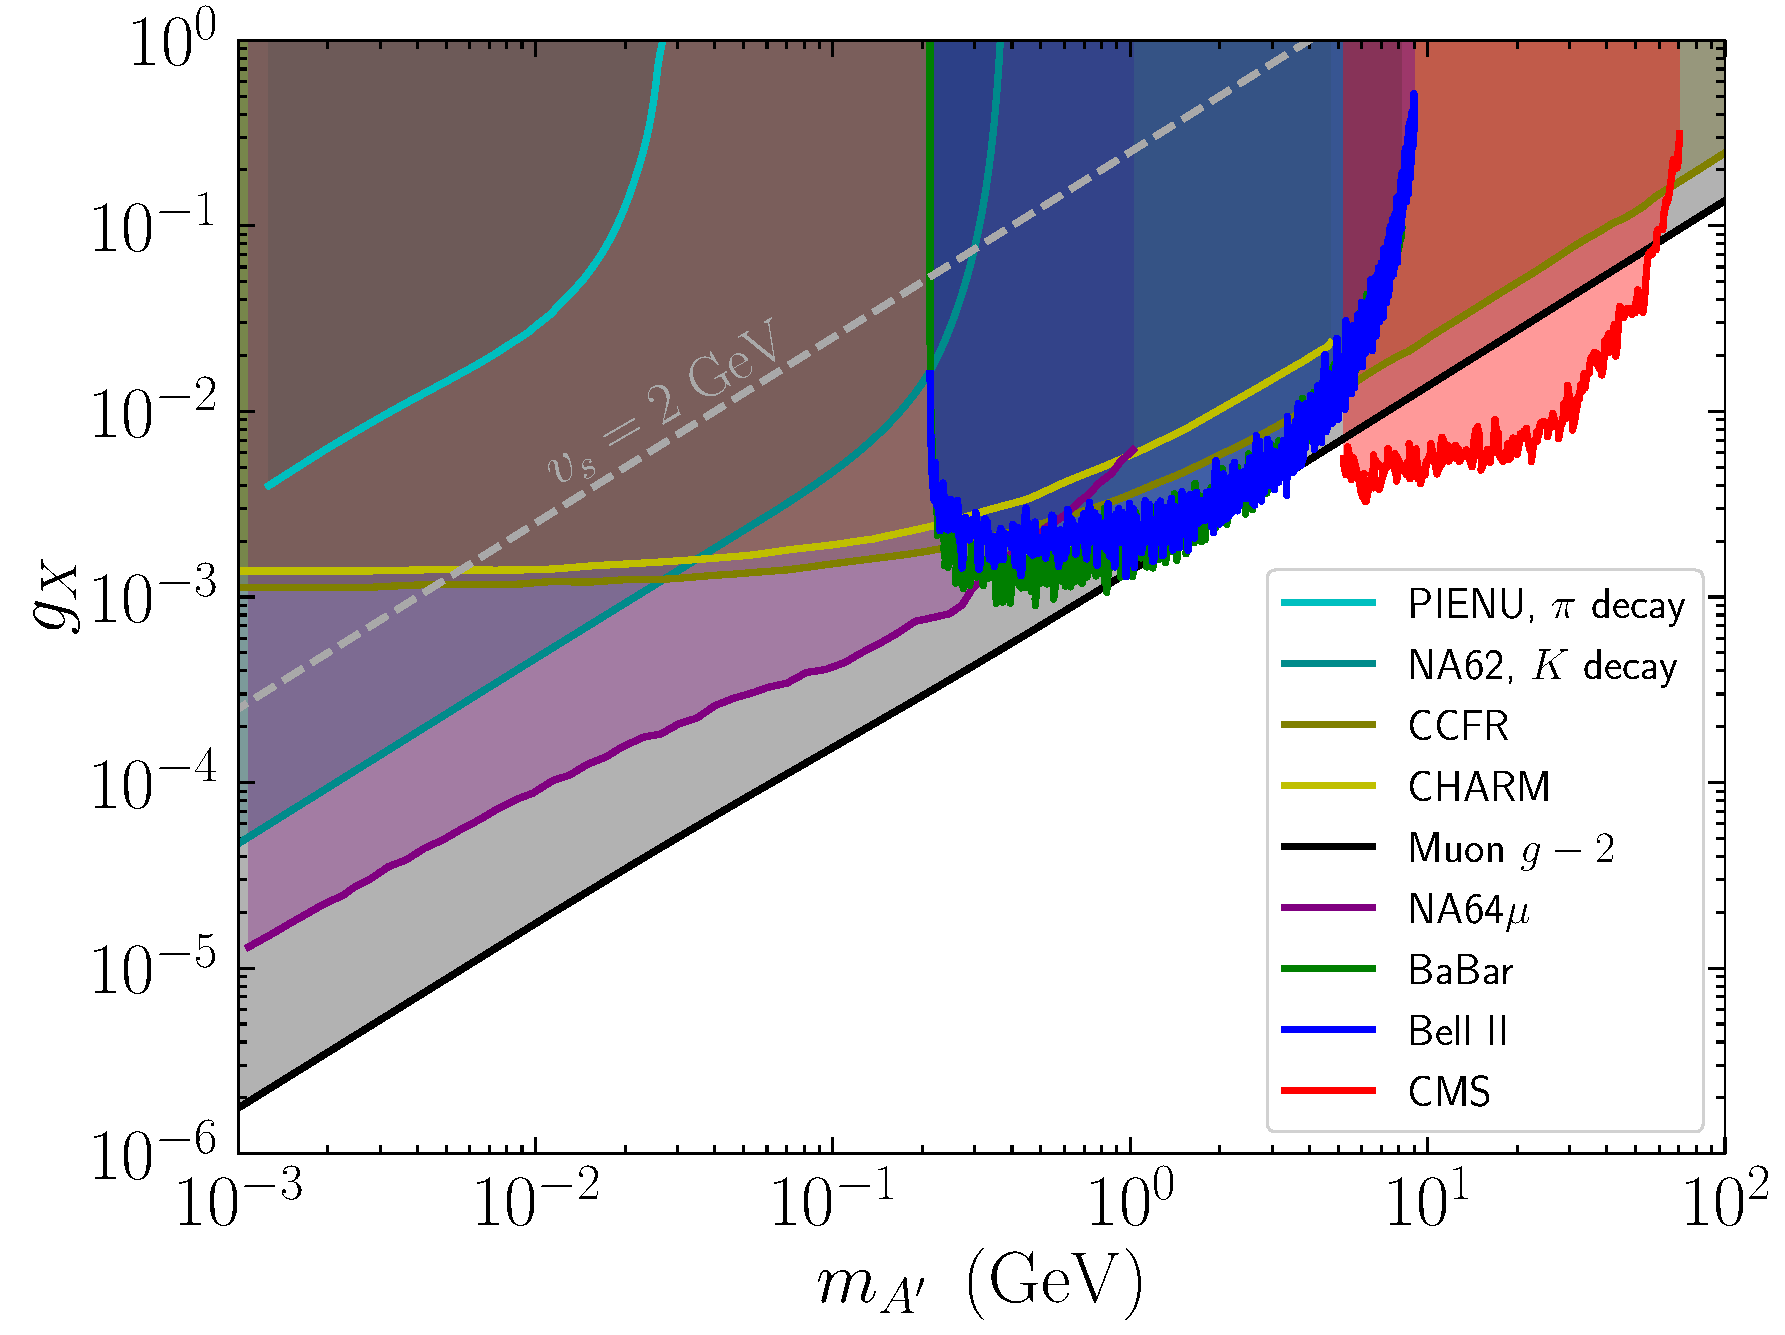
\includegraphics[width=0.48\textwidth]{plots/axial_vector_constraint}
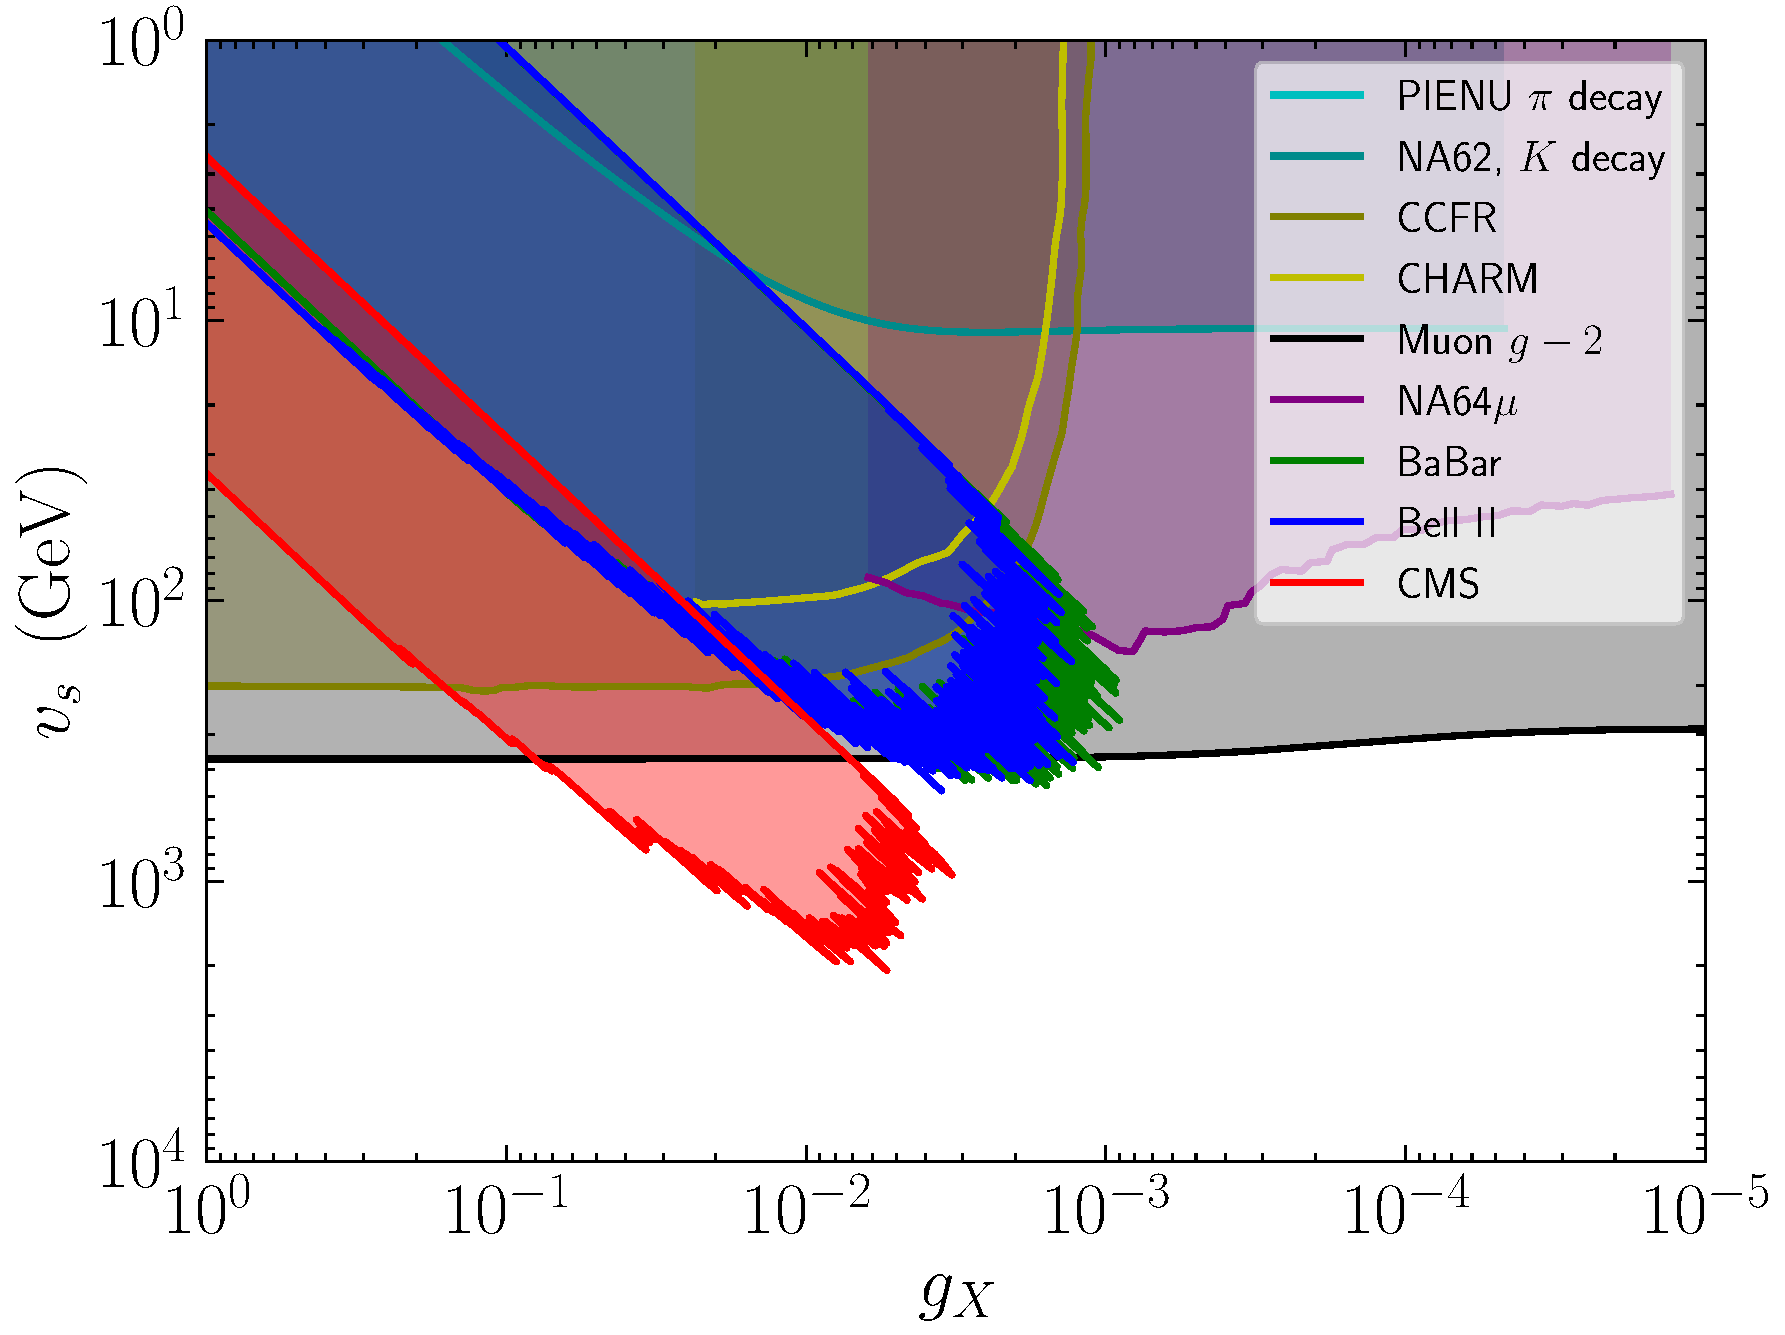
\includegraphics[width=0.48\textwidth]{plots/axial_vector_constraint_g_vs}
    \caption{Existing constraints on the axial vector model. The cyan line represents constraint from the invisible decay of pion from PIENI search~\cite{Altmannshofer:2026opc, PIENU:2021clt} and $K^+$ from NA62 search~\cite{cogollo2025constraints, gil2021search}, the yellow and olive lines represent constraints from neutrino trident process using result from CHARM~II collaboration~\cite{Altmannshofer:2014pba, geiregat1990first} and CCFR collaboration~\cite{Altmannshofer:2014pba, CCFR:1991lpl} respectively, the black line represents the constraint from measurement of muon $g-2$~\cite{Muong-2:2025xyk,Aliberti:2025beg}, the purple line repersent the constraint from the missing energy search in the muon beam dump experiment NA64$\mu$~\cite{Chakraborty:2025jbd, NA64:2024nwj}, and the green, blue and red lines represent the constraints from the $\mu^+\mu^-$ resonance search in four-muon final state in BaBar~\cite{BaBar:2016sci}, Belle~II~\cite{Belle-II:2024wtd}, and CMS~\cite{CMS:2018yxg} collaboration, respectively. Here we have $|g_X| = |Q_\ell| g_{A'} = g_{A'}$. Upper: $m_{A'} - g_X$. Lower: $g_X - v_s$.\WXP{this part need to improve }}
    \label{fig:allconstraints}
\end{figure}

\subsection{$\mu^+\mu^-$ resonance search in four-muon final state}

The axial-vector boson $A'$ can also be produced through final-state radiation (FSR) from the $\mu^+\mu^-$ pair in electron--positron annihilation~\cite{BaBar:2016sci, Belle-II:2022yaw, Belle-II:2024wtd} or in the decay of an on-shell $Z$ boson~\cite{Harigaya:2013twa, delAguila:2014soa, CMS:2018yxg}. In the parameter region of interest, the produced $A'$ will immediatly decays into a pair of charged leptons or neutrinos, leading to either a four charged lepton final state or a missing-energy signature. In this work, we focus on the four-muon channels,
\begin{equation}
	\begin{aligned}
		e^+e^- &\rightarrow \mu^+\mu^-A', \qquad A'\rightarrow \mu^+\mu^-,\\
		Z &\rightarrow \mu^+\mu^-A', \qquad A'\rightarrow \mu^+\mu^-.
	\end{aligned}
\end{equation}

The searches for these processes require the four-muon invariant mass to be consistent with the center-of-mass energy of the $e^+e^-$ collision or the $Z$ boson mass, respectively. In addition, the resonant decay $A'\to\mu^+\mu^-$ can be used to further reduce the background. Consequently, the constraints obtained from the four-muon final state are generally stronger than those from missing-energy searches based on $A'\rightarrow\nu\bar{\nu}$~\cite{Belle-II:2022yaw}. Therefore, throughout this work we consider only the limits derived from the four-muon searches.

For sufficiently heavy axial-vector bosons, the difference between vector and axial-vector FSR arises only from the longitudinal polarization of the emitted boson. This contribution is proportional to $m_\mu^2/m_{A'}^2$ and rapidly becomes negligible for $m_{A'}\gtrsim m_\mu$. As a result, the differential cross sections of vector and axial-vector radiation are nearly identical, leading to almost identical selection efficiencies after the experimental cuts. The experimental limits on the axial $U(1)_{L_\mu-L_\tau}$ model can therefore be obtained by rescaling the published limits on the corresponding vector model according to
\begin{equation}
	\begin{aligned}
		g_X^{\rm lim}(m_{A'})
		&=
		g_{\rm vec}^{\rm lim}(m_{A'})
		\left[
		\frac{\sigma_V^{\rm FSR}(g_V=1)\,
			{\rm Br}_V(\mu^+\mu^-)}
		{\sigma_A^{\rm FSR}(g_X=1)\,
			{\rm Br}_A(\mu^+\mu^-)}
		\right]^{1/2}
		\simeq
		g_{\rm vec}^{\rm lim}(m_{A'})
		\left[
		\frac{{\rm Br}_V(\mu^+\mu^-)}
		{{\rm Br}_A(\mu^+\mu^-)}
		\right]^{1/2},
		\\[2mm]
		g_X^{\rm lim}(m_{A'})
		&=
		g_{\rm vec}^{\rm lim}(m_{A'})
		\left[
		\frac{\Gamma_V^{\rm FSR}(g_V=1)\,
			{\rm Br}_V(\mu^+\mu^-)}
		{\Gamma_A^{\rm FSR}(g_X=1)\,
			{\rm Br}_A(\mu^+\mu^-)}
		\right]^{1/2}
		\simeq
		g_{\rm vec}^{\rm lim}(m_{A'})
		\left[
		\frac{{\rm Br}_V(\mu^+\mu^-)}
		{{\rm Br}_A(\mu^+\mu^-)}
		\right]^{1/2},
	\end{aligned}
	\label{eq:four-muon-rescale}
\end{equation}
where the subscripts $A$ and $V$ denote quantities in the axial and vector $U(1)_{L_\mu-L_\tau}$ models, respectively. Here $\sigma^{\rm FSR}$ denotes the cross section for $e^+e^-\rightarrow\mu^+\mu^-A'$, while $\Gamma^{\rm FSR}$ denotes the decay width for $Z\rightarrow\mu^+\mu^-A'$. The branching fraction for $A'\rightarrow\mu^+\mu^-$ is denoted by ${\rm Br}(\mu^+\mu^-)$, and $g_{\rm vec}^{\rm lim}$ represents the published exclusion limit on the gauge coupling in the vector $U(1)_{L_\mu-L_\tau}$ model.

In our analysis, we include the limits from the BaBar~\cite{BaBar:2016sci}, Belle~II~\cite{Belle-II:2024wtd}, and CMS~\cite{CMS:2018yxg} experiments. As shown in Fig.~(\ref{fig:allconstraints}), the Belle~II and BaBar searches provide constraints comparable to those from the Muon $g-2$ measurement in the mass range $0.1~\mathrm{GeV}\lesssim m_{A'}\lesssim0.4~\mathrm{GeV}$. At higher masses, the CMS search provides the strongest constraint in the region$5~\mathrm{GeV}\lesssim m_{A'}\lesssim60~\mathrm{GeV}$.\WXP{we should claim all these constraints are from the same analysis method?}

\subsection{Solar Neutrino}
As the axial vector field $A'$ also couples to left-handed neutrinos. The muon- and tau-neutrino currents can also act as a source of $A'$~\cite{Fang:2025fvo}. The resulting axial vector boson background field can influence the observed results of the Muon $g-2$ experiment, which enables the current $(g-2)_\mu$ measurement result to be used to constrain the coupling strength. 

We consider solar neutrinos as the dominant source, since they provide the largest neutrino flux at the detector location. The muon- and tau-neutrino components arise through neutrino oscillations during propagation from the Sun to the Earth.
In the relativistic limit, the axial-vector interaction to left-hand neutrinos effectively reduces to a vector-like interaction, such that the neutrino current acts as an electromagnetic-like source that generates a Yukawa potential.
Then, the potential is given by \cite{Fang:2025fvo},
\begin{equation}
A'^{\alpha} (\vec{x}_d)= \int d^3 x \sum_{\ell = e, \mu, \tau} g_X { \Phi_{\nu_\ell}^{\alpha}(x) }\frac{1}{4 \pi \Delta r}  e^{-m_{A'} \Delta r},
\label{eq:axial-vector-potential}
\end{equation}
where $x_d$ is the position of the detector, $\Phi_{\nu_\ell}^{\alpha}$ is the current of the neutrino $\nu_\ell$, and $\Delta r = |\vec{x}_d - \vec{x}|$ is the distance between the detector and the source. The induced field gives rise to a characteristic sign-changing signal: it is positive during the daytime and negative during the nighttime, superimposed on a small time-independent offset.

In the regime where the interaction range $m^{-1}_{A'}$ is larger than the distance between the Sun and Earth, the potential approaches that of a massless mediator, leading to the constraint~\cite{Fang:2025fvo}
\begin{equation}
g_X < 5.8 \times 10^{-18}\  (\text{massless limit}). 
\end{equation}
For larger mediator masses ($m_{A'} > 10^{-17}$ eV), the potential scales as $m^{-2}_{A'}$. The corresponding constraint becomes~\cite{Fang:2025fvo}
\begin{equation}
g_X < 3.1 \times   \frac{ m_{A'}}{{\rm eV}}\ (m_{A'} > 10^{-17}\ \rm{eV}). 
\end{equation}
Compared with the muon $g-2$, it is much weaker, so we don't show it in Fig. \ref{fig:allconstraints}.


\WXP{We need to discuss the results and physics of figure 1? we do not have this part?}

\section{Future Muon Collider Searches}
\label{sec:muon-collider}

A high-energy muon collider would probe the same muon-philic force in a very different mass range. Ref. \cite{Huang:2021nkl} studied the ordinary vector $L_\mu-L_\tau$ gauge boson at a benchmark $\sqrt{s}=3~{\rm TeV}$ muon collider, using both the two-body process $\mu^+\mu^-\to\ell^+\ell^-$ and an initial photon emission process $\mu^+\mu^-\to\gamma A'$. 
The former is most useful for the off-shell or near-resonance distortion of angular distributions, while the latter is the leading on-shell search strategy for $m_{A'}<\sqrt{s}$ and in the ultra-relativistic limit, its inclusive rate is only mildly sensitive to whether the charged-lepton current is vector or axial. Therefore, in this paper, we briefly discuss the possible asymmetry detection of the former channel at the future muon collider. An explicit and extensive similar discussion of dedicated comprehensive detector-level searches are refrained here, as their analysis frameworks are identical to those laid out in Ref. \cite{Huang:2021nkl}.
\begin{figure}[htbp]
\centering
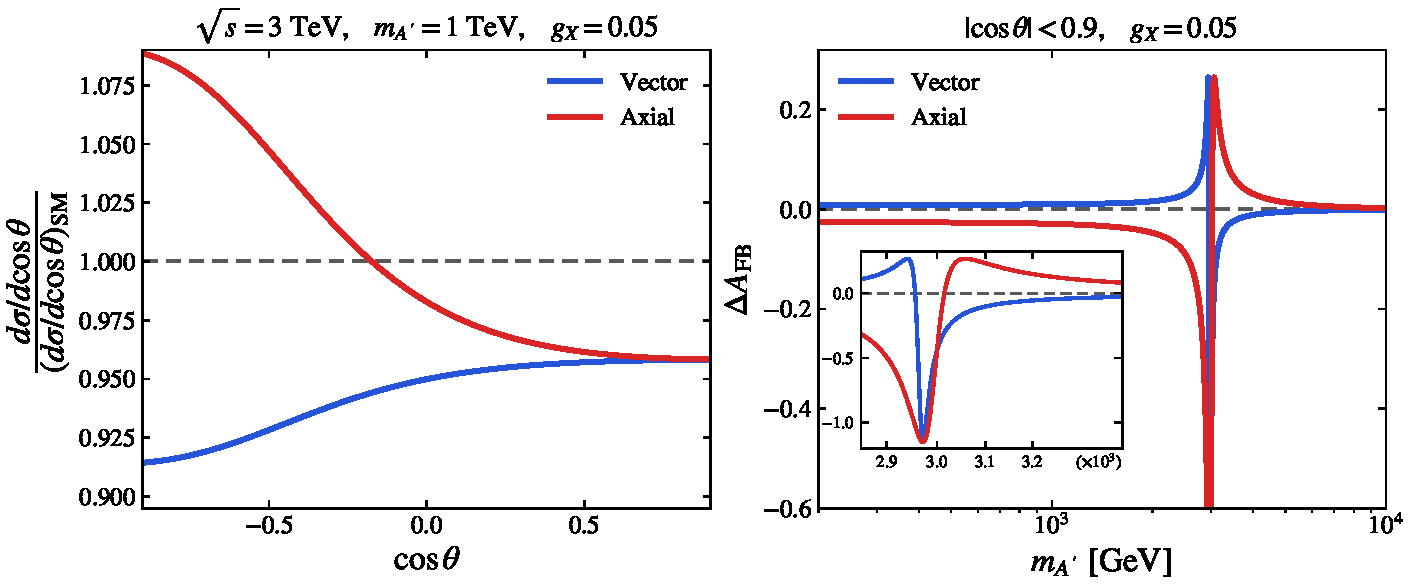
\includegraphics[width=0.94\textwidth]{plots/muon_collider_axial_vector_angular.pdf}
\caption{Future muon-collider angular comparison for $\mu^+\mu^-\to\tau^+\tau^-$ at $\sqrt{s}=3~{\rm TeV}$. Left: ratio of the differential cross section to the SM prediction for $m_{A'}=1~{\rm TeV}$ and $g'=g_X=0.05$. Right: shift in $A_{\rm FB}$, integrated over $|\cos\theta|<0.9$, as a function of $m_{A'}$. The calculation uses the massless chiral-amplitude formula in Eq.~\eqref{eq:mucollider-chiral-xsec}; the sharp structure near $m_{A'}\simeq\sqrt{s}$ is the expected $s$-channel resonance region.}
\label{fig:muon-collider-angular}
\end{figure}

For the two-body process $\mu^+\mu^-\to\ell^+\ell^-$, the ditau final state receives only $s$-channel $\gamma,Z,A'$ exchange and therefore gives the cleanest analytic illustration of the axial interference. 
Neglecting external lepton masses, the unpolarized differential cross section can be written in terms of chiral amplitudes as
\begin{align}
\frac{d\sigma_{\ell\ell}}{d\cos\theta}=
\frac{s}{128\pi}
\bigg[ \left(|\mathcal A_{LL}|^2+|\mathcal A_{RR}|^2\right)(1+\cos\theta)^2 + \left(|\mathcal A_{LR}|^2+|\mathcal A_{RL}|^2\right)(1-\cos\theta)^2 \bigg],
\label{eq:mucollider-chiral-xsec}
\end{align}
with
\begin{equation}
\mathcal A_{ij}
=\frac{e^2}{s}+\frac{g_i^Z g_j^Z}{s-m_Z^2+i m_Z\Gamma_Z}+\frac{g_i^\mu g_j^\tau}{s-m_{A'}^2+i m_{A'}\Gamma_{A'}},
\qquad i,j=L,R .
\label{eq:mucollider-chiral-amplitude}
\end{equation}
We can see that, the coupling combinations $g_i^\mu g_j^\tau$ for the vector and axial vector $U(1)_{L_\mu-L_\tau}$ are different. For comparison, the ordinary vector and our axial charge assignments are listed in Tab. \ref{tab:vector-axial-charges}. 
\begin{table}[htbp]
    \centering
    \begin{tabular}{c|cccc}
    \hline
     & $g_L^\mu$ & $g_R^\mu$ & $g_L^\tau$ & $g_R^\tau$ \\
    \hline
    vector & $g_X$ & $g_X$ & $-g_X$ & $-g_X$ \\
    axial & $g_X$ & $-g_X$ & $-g_X$ & $g_X$ \\
    \hline
    \end{tabular}
    \caption{Chiral coupling constants for left- and right-handed charged-current interactions for vector and axial vector $U(1)_{L_\mu-L_\tau}$ models.}
    \label{tab:vector-axial-charges}
\end{table}
From this table, and combined with Eqs. \eqref{eq:mucollider-chiral-xsec} and \eqref{eq:mucollider-chiral-amplitude}, we can immediately see that a total-rate reinterpretation of the vector analysis does not capture the main axial effect. To capture this axial effect, we can take forward–backward asymmetry method, which is characterized as
\begin{equation}
A_{\rm FB}=
\frac{\sigma_{\ell\ell}(\cos\theta>0)-\sigma_{\ell\ell}(\cos\theta<0)}
{\sigma_{\ell\ell}(\cos\theta>0)+\sigma_{\ell\ell}(\cos\theta<0)}.
\label{eq:mucollider-afb}
\end{equation}
As an example, in Fig.~\ref{fig:muon-collider-angular}, this effect is illustrated. For $m_{A'}=1~{\rm TeV}$ and $g_X=0.05$, the vector benchmark changes the $|\cos\theta|<0.9$ total rate by about $5\%$, while the axial benchmark changes it by only about $2\%$. Conversely, the axial case shifts $A_{\rm FB}$ by $\Delta A_{\rm FB}\simeq-2.9\times10^{-2}$, larger than the vector shift in this benchmark. By implementing angular-bin or asymmetry analysis, the constraints on this axial $U(1)_{L_\mu-L_\tau}$ model can be derived for heavy $A'$, which makes the future collider channel complementary to the low-energy probes above. As outlined at the start of this section, robust exclusion limits require detailed detector-level Monte Carlo simulations. Such a treatment would largely replicate the analysis procedure of Ref. \cite{Huang:2021nkl}. For this reason, we omit a full collider simulation in present work and present a novel feasible search method instead.


\section{Conclusion}
\label{sec:conclusion}

In this work, we have constructed an anomaly-free and renormalizable axial $U_A(1)_{L_\mu-L_\tau}$ model. Since the charge assignment forbids the diagonal SM Yukawa operators, a singlet scalar and heavy vector-like leptons generate the charged-lepton masses through a universal-seesaw-like mechanism. After diagonalizing the mass matrices, we find that the heavy-lepton limit recovers the SM Higgs Yukawa couplings and leaves a dominantly axial light-lepton current, with only an $\mathcal O(\theta_R^2)$ vector admixture. The benchmark choice $y_{\mu\tau}=0$ is both compatible with charged-lepton-flavor-violation bounds and technically natural in the presence of an approximate family symmetry.
\zb{}

In the pure-axial limit, we derived and reinterpreted the leading constraints summarized in Fig.~\ref{fig:allconstraints}. For neutrino trident production, the full finite-$m_\mu$ calculation shows that the mediator shifts $C_A$, rather than $C_V$ as in the vector benchmark. Muon beam-dump production and $(g-2)_\mu$ are particularly sensitive to the longitudinal enhancement associated with axial-current nonconservation; the NA64$_\mu$ contour is therefore presented as a rate-level phenomenological recast, while $(g-2)_\mu$ acts as a consistency bound. Invisible pion decay probes the complementary region below the kinematic endpoint. By contrast, for $m_{A'}\gg m_\mu$, axial and vector final-state-radiation rates converge, allowing the BaBar, Belle~II, and CMS four-muon limits to be reinterpreted through a controlled branching-ratio rescaling.

At a future muon collider, radiative return remains an efficient on-shell search, whereas the angular distribution of $\mu^+\mu^-\to\tau^+\tau^-$ provides a direct discriminator of the interaction structure. The axial contribution is more clearly exposed through angular bins or the forward--backward asymmetry than through the total rate, although a detector-level analysis is required to obtain a robust exclusion. Overall, an axial $L_\mu-L_\tau$ force cannot be obtained by simply replacing $g_V$ with $g_A$ in the conventional benchmark: its low-energy behavior is tied to charged-lepton mass generation and axial-current nonconservation, while vector-to-axial rescaling is justified only for selected high-energy observables.



\section{Acknowledgments}
The work of J.G. is supported by the Postdoctoral Fellowship Program (Grade C) of China Postdoctoral Science Foundation under Grant No. GZC20252775.
The work of J.L. is supported by the National Science Foundation of China under Grant No. 12235001, No. 12475103
and State Key Laboratory of Nuclear Physics and Technology under Grant No. NPT2025ZX11. 
The work of X.P.W. is supported by National Science Foundation of China under Grant No. 12375095, and the Fundamental Research Funds for the Central Universities.
J.L. and X.P.W. thank the Asia Pacific Center for Theoretical Physics (APCTP), Pohang, Korea, for their hospitality during the focus program [APCTP-2025-F01], from which this work greatly benefited. J.L. and X.P.W. also thank the Mainz Institute for Theoretical Physics (MITP) of the PRISMA+ Cluster of Excellence (Project ID 390831469) for its hospitality and partial support during the completion of this work. We also acknowledge with appreciation the valuable discussions and insights provided by the members of the Collaboration of Precision Testing and New Physics.

\bibliographystyle{JHEP}
\bibliography{references}

\end{document}
